\documentclass[11pt, a4paper]{article}

\usepackage[a4paper, margin=2.3cm]{geometry}
\usepackage[utf8]{inputenc}
\usepackage[T1]{fontenc}
\usepackage{lmodern}
\usepackage{microtype}
\usepackage{amsmath, amssymb, amsthm}
\usepackage{booktabs}
\usepackage{tabularx}
\usepackage{array}
\usepackage{multirow}
\usepackage{enumitem}
\usepackage{graphicx}
\usepackage{cite}
\usepackage{algorithm}
\usepackage{algpseudocode}
\usepackage{tikz}
\usepackage{pgfplots}
\pgfplotsset{compat=1.16}
\usetikzlibrary{arrows.meta, positioning, shapes.geometric, fit, calc}
\usepackage{caption}
\usepackage{hyperref}
\captionsetup{font=small, skip=4pt}
\renewcommand{\topfraction}{0.9}
\renewcommand{\bottomfraction}{0.8}
\renewcommand{\textfraction}{0.1}
\renewcommand{\floatpagefraction}{0.7}
\setlength{\textfloatsep}{8pt plus 2pt minus 2pt}
\setlength{\floatsep}{8pt plus 2pt minus 2pt}
\setlength{\intextsep}{8pt plus 2pt minus 2pt}

\hypersetup{
    colorlinks=true,
    linkcolor=blue,
    citecolor=blue,
    urlcolor=blue
}

\setlist{nosep, leftmargin=1.5em}
\newtheorem{proposition}{Proposition}
\newtheorem{remark}{Remark}

\newcommand{\valid}{\texttt{<|step\_\allowbreak valid|>}}
\newcommand{\invalid}{\texttt{<|step\_\allowbreak invalid|>}}
\newcommand{\soldpo}{USC-DPO-S1}

\title{\textbf{Learning to Verify: Self-Verification Training for Small Reasoning Models}}

\author{
    \textbf{Dinh-Hong Vu}$^{1[0000-0001-8513-3942]}$,
    \textbf{Tran Trung Tam}$^{2*}$,
    \textbf{Vu Minh Quan}$^{2*}$\\
    \small $^{1}$ Information Technology Project Research Team,\\
    \small Faculty of Information Technology, Ton Duc Thang University, Ho Chi Minh City, Vietnam\\
    \small $^{2}$ Faculty of Information Technology, Ton Duc Thang University, Ho Chi Minh City, Vietnam\\
    \small \texttt{vudinhhong@tdtu.edu.vn}, \texttt{520H0678@student.tdtu.edu.vn}, \texttt{522H0172@student.tdtu.edu.vn}\\
    \small $^*$Corresponding authors: \texttt{520H0678@student.tdtu.edu.vn}, \texttt{522H0172@student.tdtu.edu.vn}
}
\date{}

\begin{document}

\maketitle

\begin{abstract}
Small Language Models (SLMs) are attractive for on-device deployment, yet they fail on multi-step reasoning because errors compound along the chain of thought. External verifiers roughly double resident memory and add latency, and prompted self-correction is unreliable and verbose. We specify USC-DPO (Unified Step-Filtered Contrastive Direct Preference Optimization), a framework that places the \textit{Solve}, \textit{Verify} and \textit{Correct} phases in a single set of weights. Its components are discrete status tokens emitted after each step, Hard Context Truncation of rejected steps in the KV cache, and the Local Contrastive Preference (LCP) procedure, which turns the model's own solutions into step-aligned pairs for content and balanced pairs for verification. We revise our earlier objective, which attached the error tag to the rejected sample and therefore taught the model \emph{not} to flag its errors, and we give a finite-budget analysis that links verifier recall and false-alarm rate to end-to-end accuracy. USC-DPO is implemented in stages, and this report evaluates Stage~1 (\soldpo{}) on Qwen2.5-Math-1.5B. Stage~1 contains the data-recycling and preference-training pipeline only: solution-level pairs trained with standard DPO, without status tokens or truncation, so it is not yet a test of self-verification. In the larger pilot (146 pairs, 100 GSM8K test problems), \soldpo{} scores 68\% against 65\% for SFT-CoT ($p=0.45$). Its relative weight change is only about $10^{-4}$, its DPO loss stays at $\ln 2$, and 68 of 100 outputs are identical to those of its initialization. Two further findings matter for the next stage. A strict answer parser credits the base model with 14\% where a content-based blind grader gives 74\%. The arithmetic step checker used to build reasoning-correction pairs mislabeled 24 of 25 valid solutions as invalid. We report the pilots as validation of the pipeline and its measurement, and we specify the configuration, sample size and ablations for Stages~2 and~3.
\end{abstract}

\noindent\textbf{Keywords:} Small Language Models, Chain-of-Thought, Self-Verification, Self-Correction, Direct Preference Optimization (DPO), Step-level preference learning.

%==============================================================
\section{Introduction}
%==============================================================
Deploying Small Language Models (SLMs, here: fewer than 13B parameters) on local hardware reduces cost and keeps user data private. On multi-step reasoning with Chain-of-Thought (CoT) prompting, however, SLMs fail disproportionately: one faulty intermediate step corrupts every step that depends on it~\cite{wei2022chain}. We call this \emph{compounding error} and quantify it in Section~\ref{sec:prelim}.

Two remedies dominate. The first adds an external verifier, an outcome reward model~\cite{cobbe2021training} or a process reward model (PRM)~\cite{lightman2023let, wang2024mathshepherd}, to rerank samples or guide search. Accuracy improves, but generator and verifier must both be resident in memory, and many candidates must be scored. The second remedy prompts the model to critique and repair its own output. Without external feedback, models often turn correct answers into incorrect ones~\cite{huang2023large}, they are poor at locating their own errors~\cite{tyen2024llms}, and much apparent self-checking is decorative~\cite{zhao2025aha}.

A third route trains the verification skill into the generator. Recent evidence supports this direction: Chen et al.~\cite{chen2026selfverify} found that training a model only to judge its own solutions improved generation to a level comparable with generation training, whereas generation training did not improve self-judgment. USC-DPO pursues this route at step granularity. After each step the model emits a status token (\valid{} or \invalid{}). On \invalid{}, the step is removed from the KV cache and resampled. Training data come from the model's own correct and incorrect solutions.

\paragraph{Scope of this report.} USC-DPO is implemented in three stages. Stage~1 (\soldpo{}) builds preference pairs from the model's own solutions and trains with standard DPO at the level of whole solutions. Stage~2 adds step-level LCP pairs and the verification term of Eq.~\eqref{eq:usc}. Stage~3 adds status tokens and Hard Context Truncation at inference. This report evaluates Stage~1 only. Because Stage~1 uses no status tokens, no truncation and no step-level pairs, it is equivalent to standard DPO, and its results do not test the self-verification mechanism.

\paragraph{Contributions.}
\begin{enumerate}
    \item A specification of USC-DPO: the status-token protocol, decoding with truncation and a retry budget, and LCP with normalized step matching (Section~\ref{sec:method}).
    \item A corrected training objective. Our earlier formulation appended \invalid{} to the rejected sample, so DPO \emph{lowered} the probability of flagging errors. The revised objective separates a step-content term from a balanced verification term (Section~\ref{sec:loss}).
    \item An analysis of verified decoding under a finite retry budget $K$, with its assumptions stated explicitly (Proposition~\ref{prop:eff}).
    \item Two pilot runs with weight-level diagnostics, a blind content-based re-grading, an audit of the preference data, and a power analysis. Together they explain why the pilots could not detect an effect of preference training (Sections~\ref{sec:pilot}--\ref{sec:discussion}).
    \item A concrete evaluation plan for the full framework: corrected hyperparameters, sample size, ablations and success criteria (Section~\ref{sec:plan}).
\end{enumerate}

%==============================================================
\section{Related Work}
\label{sec:related}
%==============================================================
\paragraph{CoT, test-time compute and verifiers.}
Chain-of-Thought prompting~\cite{wei2022chain} elicits intermediate steps, and self-consistency~\cite{wang2023selfconsistency} votes over several sampled chains at extra inference cost. GSM8K~\cite{cobbe2021training} contains grade-school problems that need two to eight steps. Cobbe et al.\ trained outcome verifiers that rerank samples. Uesato et al.~\cite{uesato2022solving} compared process- and outcome-based feedback. Lightman et al.~\cite{lightman2023let} showed that step-level supervision (PRM800K, about 800{,}000 human step labels) beats outcome supervision for selecting among many samples, and they label only up to the first incorrect step. Math-Shepherd~\cite{wang2024mathshepherd} obtains step labels automatically by estimating, from sampled completions, whether a step can still reach the correct answer, and uses the resulting PRM for reranking and step-by-step PPO.

\paragraph{Self-correction and self-verification.}
Huang et al.~\cite{huang2023large} found that models struggle to correct reasoning without external feedback. Tyen et al.~\cite{tyen2024llms} showed that models are poor at finding reasoning errors but can correct them when given the error location. Self-Refine~\cite{madaan2023selfrefine} iterates feedback and refinement through prompting. Zhang et al.~\cite{zhang2024small} argue that small models need strong verifiers to self-correct. Stechly et al.~\cite{stechly2025selfverification} and Lu et al.~\cite{lu2025verification} document the limits of self-verification. SCoRe~\cite{kumar2025score} trains self-correction with multi-turn reinforcement learning on self-generated data.

\paragraph{Preference optimization and step-level variants.}
DPO~\cite{rafailov2023direct} learns from preference pairs without an explicit reward model. Offset-based variants require a minimum margin between chosen and rejected samples: ODPO~\cite{amini2024odpo} uses a pair-dependent offset, and SimPO~\cite{meng2024simpo} uses a target reward margin with a length-normalized, reference-free reward. For mathematical reasoning, Step-DPO~\cite{lai2024stepdpo} treats individual reasoning steps as the unit of preference, using self-generated data. Step-Controlled DPO~\cite{lu2024scdpo} builds negatives that begin to err at a specified step. RLVR with GRPO~\cite{shao2024deepseekmath} underlies DeepSeek-R1~\cite{deepseek2025r1}, and STaR~\cite{zelikman2022star} bootstraps rationales from correct answers.

\paragraph{Training models to self-verify.}
Chen et al.~\cite{chen2026selfverify} report an asymmetry between generation and self-verification. Training Qwen2.5-Instruct models with GRPO solely to judge the correctness of their own solutions matched generation training in accuracy and shortened reasoning; for the 1.5B model, average length fell from 1604 to 1227 tokens while average accuracy changed from 20.2\% to 21.7\%. Alternating verification and generation phases worked best. Their verifier judges whole solutions with a balanced correct/incorrect batch.

\paragraph{Positioning.}
The step-content part of USC-DPO is close to Step-DPO: both prefer a correct step to an incorrect one at the first point of divergence. We do not claim novelty for that component. The parts that differ are (i) an explicit, balanced verification objective on status tokens trained jointly with step content, and (ii) inference-time truncation driven by those tokens. Table~\ref{tab:positioning} summarizes.

\begin{table}[t]
\centering
\caption{Positioning of USC-DPO relative to closely related approaches.}
\label{tab:positioning}
\footnotesize
\begin{tabularx}{\textwidth}{lXccc}
\toprule
\textbf{Approach} & \textbf{Training signal} & \textbf{No ext.\ verifier} & \textbf{Step-level} & \textbf{Verification output} \\
\midrule
PRM + search~\cite{lightman2023let} & Human step labels & -- & \checkmark & separate model \\
Math-Shepherd~\cite{wang2024mathshepherd} & Automatic step labels & -- & \checkmark & separate model \\
Step-DPO~\cite{lai2024stepdpo} & Step preference pairs & \checkmark & \checkmark & none \\
SCDPO~\cite{lu2024scdpo} & Controlled-error negatives & \checkmark & \checkmark & none \\
SCoRe~\cite{kumar2025score} & Outcome reward, multi-turn RL & \checkmark & -- & revision turn \\
Self-verify RL~\cite{chen2026selfverify} & Binary judgment reward & \checkmark & -- & solution judgment \\
\textbf{USC-DPO (proposed)} & Step pairs + balanced verification pairs & \checkmark & \checkmark & status token per step \\
\bottomrule
\end{tabularx}
\end{table}

%==============================================================
\section{Preliminaries}
\label{sec:prelim}
%==============================================================
\subsection{Notation and compounding error}
Let $x$ be a problem with reference answer $a^\ast$, and $y=(s_1,\dots,s_n)$ a solution of $n$ steps with extracted answer $a(y)$. A policy $\pi_\theta$ generates $y$ autoregressively; $\pi_{\text{ref}}$ is a frozen reference policy and $\sigma$ the logistic sigmoid. If step $s_t$ is correct with probability $p_t$ given a correct prefix, and any step error invalidates the chain, then $\Pr[\text{chain correct}]=\prod_t p_t$, which equals $p^{n}$ for constant $p$ (Figure~\ref{fig:compound}). With $p=0.95$ and $n=8$ the chain is correct 66\% of the time, and with $p=0.90$ only 43\%. This illustrative model assumes independent step errors.

\begin{figure}[t]
\centering
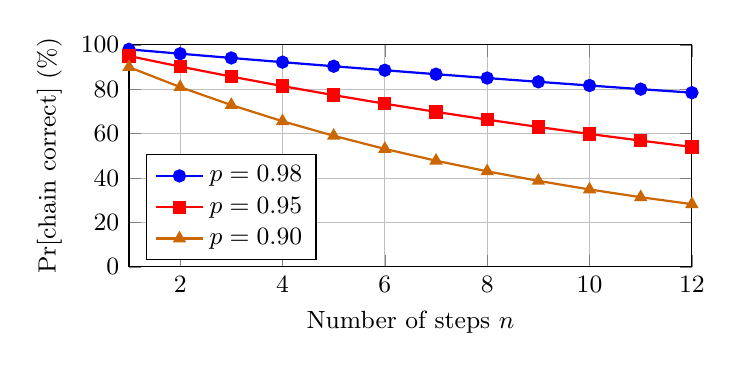
\begin{tikzpicture}
\begin{axis}[
  width=0.72\textwidth, height=4.4cm, xlabel={Number of steps $n$}, ylabel={$\Pr[\text{chain correct}]$ (\%)},
  xmin=1, xmax=12, ymin=0, ymax=100, grid=major, legend pos=south west, legend cell align=left, font=\small]
\addplot[thick, blue, mark=*, domain=1:12, samples=12] {100*0.98^x};
\addplot[thick, red, mark=square*, domain=1:12, samples=12] {100*0.95^x};
\addplot[thick, orange!80!black, mark=triangle*, domain=1:12, samples=12] {100*0.90^x};
\legend{$p=0.98$, $p=0.95$, $p=0.90$}
\end{axis}
\end{tikzpicture}
\caption{Probability that an $n$-step chain is entirely correct, $p^{n}$ (illustrative model with independent step errors).}
\label{fig:compound}
\end{figure}

\subsection{Direct Preference Optimization}
For preference tuples $(x,y_w,y_l)$ with $y_w$ preferred, DPO~\cite{rafailov2023direct} starts from the KL-regularized objective $\max_{\pi}\mathbb{E}[r(x,y)]-\beta\,\mathrm{KL}(\pi\,\|\,\pi_{\text{ref}})$, whose optimum satisfies
\[ r(x,y)=\beta\log\frac{\pi^\ast(y|x)}{\pi_{\text{ref}}(y|x)}+\beta\log Z(x). \]
Under the Bradley--Terry model the partition term cancels:
\begin{equation}
\mathcal{L}_{\text{DPO}}=-\mathbb{E}\big[\log\sigma(\beta\,\Delta_\theta)\big],\qquad
\Delta_\theta=\log\frac{\pi_\theta(y_w|x)}{\pi_{\text{ref}}(y_w|x)}-\log\frac{\pi_\theta(y_l|x)}{\pi_{\text{ref}}(y_l|x)}.
\label{eq:dpo}
\end{equation}
We call $\beta\Delta_\theta$ the \emph{preference margin}. At initialization $\pi_\theta=\pi_{\text{ref}}$, so the margin is $0$ and the loss is $\ln 2\approx 0.693$. A loss that stays near $\ln 2$ therefore means the policy has not separated chosen from rejected samples.

%==============================================================
\section{The USC-DPO Framework}
\label{sec:method}
%==============================================================
\subsection{Three-state operation}
\begin{itemize}
    \item \textbf{Solve:} generate the next candidate step $s_t$.
    \item \textbf{Verify:} immediately after $s_t$, emit one status token, \valid{} or \invalid{}, instead of a free-text critique.
    \item \textbf{Correct:} on \invalid{}, purge $s_t$ and its tag and resample a step from the last verified prefix.
\end{itemize}

\begin{figure}[t]
\centering
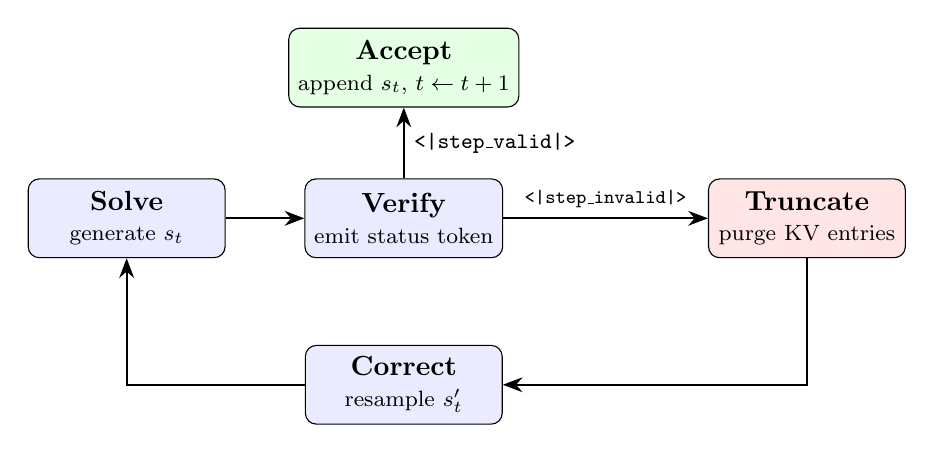
\begin{tikzpicture}[
  node distance=1.0cm,
  state/.style={draw, rounded corners, minimum width=2.5cm, minimum height=1.0cm, align=center, fill=blue!8},
  bad/.style={draw, rounded corners, minimum width=2.5cm, minimum height=1.0cm, align=center, fill=red!10},
  arr/.style={-{Stealth[length=2.5mm]}, thick}]
\node[state] (solve) {\textbf{Solve}\\[-1pt]\footnotesize generate $s_t$};
\node[state, right=of solve] (verify) {\textbf{Verify}\\[-1pt]\footnotesize emit status token};
\node[bad, right=2.6cm of verify] (trunc) {\textbf{Truncate}\\[-1pt]\footnotesize purge KV entries};
\node[state, below=1.1cm of verify] (correct) {\textbf{Correct}\\[-1pt]\footnotesize resample $s_t'$};
\node[state, above=0.9cm of verify, fill=green!10] (accept) {\textbf{Accept}\\[-1pt]\footnotesize append $s_t$, $t\leftarrow t+1$};
\draw[arr] (solve) -- (verify);
\draw[arr] (verify) -- node[above, font=\scriptsize] {\invalid} (trunc);
\draw[arr] (verify) -- node[right, font=\footnotesize] {\valid} (accept);
\draw[arr] (trunc) |- (correct);
\draw[arr] (correct) -| (solve);
\end{tikzpicture}
\caption{Closed-loop runtime of USC-DPO. A step is committed only after \valid{}; otherwise its tokens are evicted from the cache and a replacement is sampled from the last verified prefix.}
\label{fig:architecture}
\end{figure}

\subsection{Decoding with Hard Context Truncation}
Two special tokens are added to the vocabulary and always follow a step delimiter. Algorithm~\ref{alg:decode} decodes with a retry budget $K$. After $K$ attempts the last candidate is committed, so generation always terminates; the event is logged as a verification failure. Truncation discards the key-value states of the rejected step and resumes from the cached verified prefix. In a decoder-only transformer this is a crop of the cache to the verified length, not a recomputation. Rejected text never re-enters the context, so it cannot distract later steps.

\begin{algorithm}[t]
\caption{Step-level decoding with Hard Context Truncation}
\label{alg:decode}
\begin{algorithmic}[1]
\Require Problem $x$, policy $\pi_\theta$, retry budget $K$, maximum steps $T_{\max}$
\State $c \gets x$; \quad $t \gets 1$
\While{$t \le T_{\max}$ \textbf{and} not \textsc{EndOfSolution}($c$)}
    \For{$k = 1,\dots,K$}
        \State $s \gets$ \textsc{SampleStep}($\pi_\theta, c$) \Comment{Solve}
        \State $v \gets$ \textsc{SampleStatusToken}($\pi_\theta, c \oplus s$) \Comment{Verify}
        \If{$v=$ \valid{} \textbf{or} $k=K$}
            \State \textbf{break} \Comment{commit; forced commit when $k=K$}
        \EndIf
        \State \textsc{CropKVCache}($|c|$) \Comment{Truncate: restore verified prefix}
    \EndFor
    \State $c \gets c \oplus s$; \quad $t \gets t+1$
\EndWhile
\State \Return \textsc{ExtractAnswer}($c$)
\end{algorithmic}
\end{algorithm}

\subsection{LCP: Local Contrastive Preference recycling}
\label{sec:lcp}
LCP harvests training signal from the model's own samples. For each problem, several solutions are sampled and labeled by comparing the extracted answer with the reference. For every problem with at least one correct solution $P$ and one incorrect solution $N$, LCP finds the first step at which they diverge (Algorithm~\ref{alg:lcp}). The step pair is close to Step-DPO~\cite{lai2024stepdpo}. LCP adds two verification pairs per divergence, which are balanced by construction.

Exact string comparison declares equivalent but differently phrased steps divergent, which places the divergence too early. LCP therefore compares a normalized form $\textsc{Norm}(s)$: the ordered sequence of numeric values in $s$, with whitespace and units removed, falling back to lower-cased text when $s$ contains no number. This is a heuristic. Automatic step labels in the style of Math-Shepherd~\cite{wang2024mathshepherd}, which estimate whether a step can still reach the answer, are a stronger alternative that we plan to compare.

\begin{algorithm}[t]
\caption{LCP: divergence detection and pair construction}
\label{alg:lcp}
\begin{algorithmic}[1]
\Require Correct solution $P$, incorrect solution $N$ for the same problem $q$
\Ensure Step pair $(x, s_w, s_l)$ and verification pairs $\mathcal{V}$
\State $S_P \gets \textsc{SplitSteps}(P)$; \quad $S_N \gets \textsc{SplitSteps}(N)$
\State $i \gets 0$
\While{$i < \min(|S_P|, |S_N|)$ \textbf{and} $\textsc{Norm}(S_P[i]) = \textsc{Norm}(S_N[i])$}
    \State $i \gets i + 1$
\EndWhile
\If{$i = \min(|S_P|, |S_N|)$} \Return $\varnothing$ \Comment{no step-level divergence}
\EndIf
\State $x \gets q \oplus \textsc{Join}(S_P[0:i])$ \Comment{shared verified prefix}
\State $s_w \gets S_P[i]$; \quad $s_l \gets S_N[i]$ \Comment{status tag \emph{not} appended}
\State $\mathcal{V} \gets \{(x\oplus s_w,\ \valid \succ \invalid),\ (x\oplus s_l,\ \invalid \succ \valid)\}$
\State \Return $(x, s_w, s_l), \mathcal{V}$
\end{algorithmic}
\end{algorithm}

\begin{table}[t]
\centering
\caption{Pairs produced by LCP for one divergence.}
\label{tab:dpo_dataset}
\small
\begin{tabularx}{\textwidth}{lXX}
\toprule
\textbf{Pair} & \textbf{Context} & \textbf{Preference} \\
\midrule
Step content & problem $\oplus$ shared prefix & correct step $s_w$ $\succ$ incorrect step $s_l$ \\
Verification (+) & problem $\oplus$ prefix $\oplus\, s_w$ & \valid{} $\succ$ \invalid{} \\
Verification ($-$) & problem $\oplus$ prefix $\oplus\, s_l$ & \invalid{} $\succ$ \valid{} \\
\bottomrule
\end{tabularx}
\end{table}

\subsection{Training objective}
\label{sec:loss}
\paragraph{Earlier formulation and its flaw.} Our earlier version appended \invalid{} to the rejected step and added a penalty $\lambda$:
\begin{equation}
\mathcal{L}_{\text{old}}=-\mathbb{E}\Big[\log\sigma\Big(\beta\log\tfrac{\pi_\theta(s_w|x)}{\pi_{\text{ref}}(s_w|x)}-\beta\log\tfrac{\pi_\theta(s_l\oplus\invalid|x)}{\pi_{\text{ref}}(s_l\oplus\invalid|x)}-\lambda\Big)\Big].
\label{eq:old}
\end{equation}
Because $\log\pi_\theta(s_l\oplus\invalid|x)$ contains the term $\log\pi_\theta(\invalid\mid x\oplus s_l)$, and DPO pushes the rejected log-ratio \emph{down}, Eq.~\eqref{eq:old} lowers the probability of flagging an erroneous step, the opposite of the intended behavior. The constant $\lambda$ cannot fix this. With $z=\beta\Delta_\theta-\lambda$, the gradient is $-\sigma(\lambda-\beta\Delta_\theta)\,\beta\nabla_\theta\Delta_\theta$; $\lambda$ rescales the weight of each pair but leaves the direction of the update unchanged. Such an offset is the mechanism already studied in ODPO~\cite{amini2024odpo} and in the target margin of SimPO~\cite{meng2024simpo}, so we treat it as an optional hyperparameter rather than a contribution.

\paragraph{Revised objective.} USC-DPO separates step content from verification:
\begin{equation}
\mathcal{L}_{\text{USC}}=\underbrace{-\mathbb{E}_{(x,s_w,s_l)}\big[\log\sigma(\beta\,\Delta^{\text{step}}_\theta-\delta)\big]}_{\text{step content}}
\;\underbrace{-\;\mu\,\mathbb{E}_{(c,v_w,v_l)\in\mathcal{V}}\big[\log\sigma(\beta_v\,\Delta^{\text{ver}}_\theta)\big]}_{\text{verification}},
\label{eq:usc}
\end{equation}
where $\Delta^{\text{step}}_\theta$ is the DPO log-ratio difference of Eq.~\eqref{eq:dpo} computed on step tokens only, $\Delta^{\text{ver}}_\theta=\log\frac{\pi_\theta(v_w|c)}{\pi_{\text{ref}}(v_w|c)}-\log\frac{\pi_\theta(v_l|c)}{\pi_{\text{ref}}(v_l|c)}$ is computed on the single status token, $\delta\ge 0$ is an optional ODPO-style offset, and $\mu$ weights the verification term. Because $\mathcal{V}$ contains one positive and one negative example per divergence, the verification data are balanced, which Chen et al.~\cite{chen2026selfverify} found important for verification training. A token-level cross-entropy on the status token is a simpler alternative to the second term; we will compare both.

\subsection{Analysis of verified decoding with a finite budget}
\label{sec:analysis}
Let $p$ be the per-step accuracy of the generator, and describe the verifier by its \emph{recall} $r=\Pr[\invalid\mid\text{step wrong}]$ and \emph{false-alarm rate} $f=\Pr[\invalid\mid\text{step correct}]$. The metric FPR-V (Section~\ref{sec:plan}) equals $1-r$.

\begin{proposition}[Effective step accuracy with retry budget $K$]
\label{prop:eff}
Assume that attempts at a prefix are independent draws with the same $(p,r,f)$, and that Algorithm~\ref{alg:decode} commits the first accepted attempt, or the $K$-th attempt if all are rejected. Let $a=p(1-f)+(1-p)(1-r)$ be the per-attempt acceptance probability and $q=1-a$. Then the committed step is correct with probability
\begin{equation}
p_{\text{eff}}(K)=p(1-f)\,\frac{1-q^{K-1}}{1-q}+q^{K-1}p,
\label{eq:peff}
\end{equation}
and the expected number of attempts is $(1-q^{K})/(1-q)$. In particular $p_{\text{eff}}(1)=p$, and $p_{\text{eff}}(K)\to p(1-f)/a$ as $K\to\infty$.
\end{proposition}
\begin{proof}
Attempt $k<K$ is committed if the first $k-1$ attempts were rejected and attempt $k$ is accepted; it is then correct with probability $p(1-f)$. Summing $q^{k-1}p(1-f)$ over $k=1,\dots,K-1$ gives the first term. If the first $K-1$ attempts are rejected (probability $q^{K-1}$), attempt $K$ is committed regardless of its tag and is correct with probability $p$. The expected number of attempts is $\sum_{k=1}^{K}q^{k-1}$.
\end{proof}

\begin{table}[t]
\centering
\caption{Proposition~\ref{prop:eff} for $p=0.90$ and $n=8$ steps; chain accuracy is $p_{\text{eff}}^{8}$ (\%). Without verification ($K=1$) it is 43.0\%. Values in parentheses are expected attempts per step.}
\label{tab:analytic}
\small
\begin{tabular}{ccccc}
\toprule
Recall $r$ & False alarm $f$ & $K=2$ & $K=3$ & $K\to\infty$ \\
\midrule
0.50 & 0.10 & 58.9 (1.14) & 61.5 (1.16) & 61.9 (1.16) \\
0.70 & 0.05 & 71.2 (1.12) & 75.3 (1.13) & 75.9 (1.13) \\
0.90 & 0.05 & 82.7 (1.14) & 89.9 (1.15) & 91.1 (1.16) \\
0.95 & 0.02 & 87.7 (1.11) & 94.7 (1.13) & 95.6 (1.13) \\
\bottomrule
\end{tabular}
\end{table}

Table~\ref{tab:analytic} shows that a small budget ($K=3$) recovers most of the asymptotic gain, and that the gain is governed mainly by recall.

\begin{remark}[Assumptions]
\label{rem:assump}
Generator and verifier are the same model, so a step the model gets wrong is also one it may fail to detect. This correlation is absorbed into $r$ and $f$ \emph{provided they are measured on the model's own steps}, which is how FPR-V is defined. The stronger assumption is independence across retries. Resampling at the same prefix tends to repeat the same misconception, so retries are positively correlated, and Eq.~\eqref{eq:peff} should be read as an optimistic estimate. A model in which a prefix is ``hard'' with some probability, and all retries at a hard prefix fail, would give a strictly smaller $p_{\text{eff}}$. Proposition~\ref{prop:eff} is therefore used to set targets for $r$ and $f$, not to predict accuracy.
\end{remark}

\paragraph{Memory and token cost.} An external verifier of the same size doubles resident weights (for 1.5B parameters in 16-bit precision, about 3~GB to 6~GB before KV caches). The unified model keeps one copy. Status tokens cost one token per step plus the tokens of discarded attempts, instead of a free-text critique.

%==============================================================
\section{Pilot Studies: USC-DPO Stage~1}
\label{sec:pilot}
%==============================================================
\subsection{What the pilots test}
Two pilot runs exercise the data-recycling, training and evaluation pipeline on a single Tesla T4 GPU. Both runs evaluate Stage~1 of USC-DPO (\soldpo{}), not the full framework (Table~\ref{tab:status}). In Stage~1 the preference-trained model is standard DPO on solution-level pairs. \textbf{Run~A} (October) is the configuration criticized in the first review of this report. \textbf{Run~B} (November) retrains SFT-CoT on the full training set with a larger learning rate, rebuilds the preference data with an arithmetic step checker, and doubles the test set. Run~B is the main pilot below, and Run~A serves as a reference point.

\begin{table}[t]
\centering
\caption{Full framework versus the Stage~1 configuration evaluated in the two pilot runs.}
\label{tab:status}
\small
\begin{tabularx}{\textwidth}{lXX}
\toprule
\textbf{Component} & \textbf{Full USC-DPO (Stages 1--3)} & \textbf{Pilots (Stage~1, \soldpo{})} \\
\midrule
Status tokens, truncation & yes & no \\
Pair granularity & step pairs + verification pairs & whole solutions \\
Chosen sample & model's own correct step & GSM8K reference solution (except Run~A step-efficiency pairs) \\
Objective & Eq.~\eqref{eq:usc} & standard DPO, Eq.~\eqref{eq:dpo} \\
Scale & thousands of problems & Run~A: 81 pairs / 48 problems; Run~B: 146 pairs / 68 problems \\
Evaluation & full GSM8K test, MATH-500, $\ge 3$ seeds & Run~A: 50 problems; Run~B: 100 problems; 1 seed \\
\bottomrule
\end{tabularx}
\end{table}

\subsection{Data and training}
Both runs use Qwen2.5-Math-1.5B~\cite{yang2024qwen25math} with LoRA~\cite{hu2022lora} ($r=8$, $\alpha=16$, dropout 0.05, q and v projections; 1{,}089{,}536 trainable parameters, about 0.07\%). Table~\ref{tab:hparams} lists the differences.

\textbf{Run~B data.} The first 80 GSM8K training problems are held out as a preference pool, and the remaining 7{,}393 solutions train SFT-CoT. The SFT-CoT model samples four solutions per pool problem (temperature 0.85, top-$p$ 0.95, at most 384 new tokens), giving 320 candidates: 186 with a correct final answer, 126 incorrect and 8 unreadable. A rule-based step checker evaluates explicit arithmetic equalities in each of the 1{,}392 deduplicated steps and labels a step \texttt{UNKNOWN} when it finds no checkable equality (611 steps). Two pair types are built. \emph{Answer-correction} pairs (121) prefer the GSM8K reference solution to a sampled solution with a wrong answer. \emph{Reasoning-correction} pairs (25) prefer the reference solution to a sampled solution that has the correct answer but contains an equality the checker marked false. The 146 pairs come from 68 problems, and no step-efficiency pair passed the filter.

\begin{table}[t]
\centering
\caption{Pilot training configurations.}
\label{tab:hparams}
\small
\begin{tabular}{lll}
\toprule
\textbf{Setting} & \textbf{Run~A} & \textbf{Run~B} \\
\midrule
SFT-CoT data / steps & 100 solutions / 25 & 7{,}393 solutions / 1{,}849 \\
SFT-CoT learning rate & $2\times10^{-6}$ & $1\times10^{-5}$ \\
Candidates sampled from & Base & SFT-CoT \\
Preference pairs & 61 answer-corr.\ + 20 step-eff. & 121 answer-corr.\ + 25 reasoning-corr. \\
DPO epochs / steps & 3 / 243 & 3 / 438 \\
DPO learning rate / $\beta$ & $1\times10^{-6}$ / 0.1 & $1\times10^{-6}$ / 0.1 \\
Test problems & first 50 & first 100 \\
\bottomrule
\end{tabular}
\end{table}

\subsection{Evaluation protocol}
All models answer the same problems with the same prompt, greedy decoding, repetition penalty 1.05 and at most 384 new tokens. We grade with two procedures. \emph{Strict}: the Run~B parser accepts only a \texttt{\#\#\#\#} marker, a boxed answer or a marked final line, and counts anything else as incorrect. \emph{Blind rule (v2)}: a deterministic extractor applied to all outputs in shuffled order without model identity. It takes, in order, a \texttt{\#\#\#\#} marker, a boxed answer, ``the answer is'', and otherwise the value after the last ``='' in the final sentence, or else the first number in that sentence. The v2 rule was written after inspecting Run~A failures. On Run~A it agreed with the authors' manual labels on 149 of 150 outputs (Cohen's $\kappa=0.98$), and it was then applied unchanged to Run~B. Intervals are Wilson 95\%~\cite{wilson1927probable}, and paired comparisons use the exact McNemar test~\cite{mcnemar1947note}.

%==============================================================
\section{Pilot Results}
\label{sec:results}
%==============================================================
\subsection{Accuracy and the effect of answer format}
Table~\ref{tab:acc} shows that the grader changes the conclusion. Under strict parsing, Base scores 14\% and SFT-CoT 65\%, an apparent gain of 51 points. However, 80 of the 100 Base outputs have no final-answer marker and are therefore counted as wrong. Under the blind v2 rule, Base scores 74\%, SFT-CoT 66\% and \soldpo{} 68\%. A spot check of 10 of the 60 Base outputs credited only by v2 found that each final sentence states the reference answer. The strict comparison therefore mostly measures format compliance: SFT-CoT learned to emit the marker.

\begin{table}[t]
\centering
\caption{Accuracy (\%) with Wilson 95\% intervals. Run~A: 50 problems; Run~B: 100 problems.}
\label{tab:acc}
\small
\begin{tabular}{lccc}
\toprule
\textbf{Model} & \textbf{Run~B strict} & \textbf{Run~B blind rule (v2)} & \textbf{Run~A blind rule (v2)} \\
\midrule
Base & 14 (9--22); 80 unparsed & 74 (65--82) & 74 (60--84) \\
SFT-CoT & 65 (55--74); 3 unparsed & 66 (56--75) & 74 (60--84) \\
\soldpo{} & 68 (58--76); 2 unparsed & 68 (58--76) & 74 (60--84) \\
\bottomrule
\end{tabular}
\end{table}

None of the paired differences is significant (Table~\ref{tab:paired}). \soldpo{} and SFT-CoT disagree on only 6 or 7 problems, and the direction favoring \soldpo{} rests on 5 versus 2 (strict) or 4 versus 2 (v2) problems. Under v2, Base is ahead of SFT-CoT on 14 problems and behind on 6 ($p=0.12$), so the content-graded evidence does not support the claim that SFT-CoT improved reasoning over Base.

\begin{table}[t]
\centering
\caption{Run~B paired comparisons: problems solved by A only and by B only, with exact McNemar $p$.}
\label{tab:paired}
\small
\begin{tabular}{lcc}
\toprule
\textbf{A vs.\ B} & \textbf{Strict} & \textbf{Blind rule (v2)} \\
\midrule
\soldpo{} vs.\ SFT-CoT & 5 / 2, $p=0.45$ & 4 / 2, $p=0.69$ \\
SFT-CoT vs.\ Base & -- & 6 / 14, $p=0.12$ \\
\soldpo{} vs.\ Base & -- & 8 / 14, $p=0.29$ \\
\bottomrule
\end{tabular}
\end{table}

\subsection{Training dynamics}
In Run~B the DPO loss ranged from 0.642 to 0.756 over 438 steps, and the epoch means were 0.6967, 0.6962 and 0.6938, all at $\ln 2$ (Table~\ref{tab:train}). The mean margin was negative in every epoch, and it was positive in only 200 of 438 steps (45.7\%). The policy did not learn to prefer the chosen samples. Run~A showed the same pattern (epoch means 0.6925, 0.6924, 0.6935; margin positive in 53.1\% of steps).

\begin{table}[t]
\centering
\caption{Run~B DPO training: mean loss, mean margin and fraction of steps with positive margin (146 steps per epoch).}
\label{tab:train}
\small
\begin{tabular}{cccc}
\toprule
\textbf{Epoch} & \textbf{Mean loss} & \textbf{Mean margin} & \textbf{Positive-margin steps} \\
\midrule
1 & 0.6967 & $-0.0067$ & 42.5\% \\
2 & 0.6962 & $-0.0058$ & 46.6\% \\
3 & 0.6938 & $-0.0009$ & 47.9\% \\
\bottomrule
\end{tabular}
\end{table}

\subsection{Did the adapters change the model?}
For each adapted matrix the LoRA update is $\Delta W=\tfrac{\alpha}{r}BA$. Table~\ref{tab:diag} compares $\|\Delta W\|_F$ with $\|W\|_F$ for the q and v projections of layers 0, 9, 18 and 27. Raising the SFT learning rate to $10^{-5}$ and using the full training set increased the relative SFT update about 370-fold, from $2.4\times10^{-5}$ to $8.8\times10^{-3}$. This change is visible in behavior: no Run~B SFT-CoT output is identical to Base, the mean length fell from 204 to 112 tokens, and unparsed outputs fell from 80 to 3. The DPO learning rate stayed at $10^{-6}$, and the DPO update stayed at about $10^{-4}$ in both runs. In Run~B, 68 of 100 \soldpo{} outputs are character-identical to those of its SFT-CoT initialization. With Adam, a learning rate of $10^{-6}$ bounds the change of each parameter to about $10^{-6}$ per step, so 438 steps cannot move $B$, which starts at zero, beyond about $4\times10^{-4}$. The observed maximum is $2.8\times10^{-4}$. LoRA fine-tuning typically uses learning rates on the order of $10^{-4}$~\cite{dettmers2023qlora}.

\begin{table}[t]
\centering
\caption{Size of the learned updates and output agreement. Relative change is $\|\Delta W\|_F/\|W\|_F$ over eight sampled q/v matrices (mean).}
\label{tab:diag}
\small
\begin{tabular}{lcccc}
\toprule
 & \multicolumn{2}{c}{\textbf{Run~A}} & \multicolumn{2}{c}{\textbf{Run~B}} \\
\cmidrule(lr){2-3}\cmidrule(lr){4-5}
 & SFT-CoT & \soldpo{} & SFT-CoT & \soldpo{} \\
\midrule
Relative change & $2.4\times10^{-5}$ & $1.0\times10^{-4}$ & $8.8\times10^{-3}$ & $1.3\times10^{-4}$ \\
Outputs identical to the model it starts from & 33/50 & 26/50 & 0/100 & 68/100 \\
\bottomrule
\end{tabular}
\end{table}

\subsection{Quality of the preference data}
We re-checked the 25 reasoning-correction pairs by evaluating every equality in the rejected solutions after removing currency signs and thousands separators and reading ``x'' and ``\%'' as multiplication and percent. In 24 of the 25 rejected solutions every equality is arithmetically true. The checker had parsed, for example, ``2 x 12 = 24'' as ``12 = 24'' and ``\$10 + \$20 + \$30 = 60'' as ``30 = 60''. Only one rejected solution contains a genuinely malformed equality (``40/100 = 636''), and all 25 reach the correct final answer. These pairs therefore teach the model to disprefer valid solutions. In addition, every chosen sample in Run~B, and every answer-correction chosen sample in Run~A, is a GSM8K reference solution rather than a sample from the model being trained. Step-DPO reports that self-generated chosen data is more effective than data from humans or GPT-4 for DPO, which it attributes to their out-of-distribution nature~\cite{lai2024stepdpo}. Both issues weaken the preference signal independently of the learning rate.

\subsection{Efficiency}
In Run~B mean latency is 8.6~s for Base and 6.2--6.3~s for the adapter models, but only because their outputs are about half as long. Per generated token, the adapter models are slower (0.056~s versus 0.042~s, about 31\%). Both adapter models are evaluated as unmerged PEFT wrappers, which add two low-rank products per adapted projection at each decoding step. LoRA adds no inference latency once merged~\cite{hu2022lora}, so this overhead most likely comes from the evaluation setup and not from the models. We did not measure merged latency.

\subsection{Statistical power}
For a paired comparison, the number of problems needed to detect an accuracy difference $d$ at $\alpha=0.05$ with 80\% power is about $n\approx(z_{0.975}\sqrt{\pi_d}+z_{0.8}\sqrt{\pi_d-d^2})^2/d^2$, where $\pi_d$ is the fraction of discordant problems. In Run~B, \soldpo{} and SFT-CoT disagree on 6--7\% of problems. With $n=100$ and $\pi_d=0.06$, the minimum detectable difference is about 7 points, more than twice the observed 2--3 points. Table~\ref{tab:power} shows that detecting a 3-point difference needs roughly 520--870 problems, which the full GSM8K test set (1{,}319) provides.

\begin{table}[t]
\centering
\caption{Approximate number of problems for a paired test to detect difference $d$ ($\alpha=0.05$, power 0.8).}
\label{tab:power}
\small
\begin{tabular}{lccc}
\toprule
Discordance $\pi_d$ & $d=2$ points & $d=3$ points & $d=5$ points \\
\midrule
0.06 & 1{,}175 & 521 & 186 \\
0.10 & 1{,}960 & 870 & 312 \\
\bottomrule
\end{tabular}
\end{table}

%==============================================================
\section{Discussion}
\label{sec:discussion}
%==============================================================
\paragraph{What the pilots show.} Run~B confirms the review's diagnosis. Raising the SFT learning rate made SFT-CoT change behavior substantially, mainly in format and length. Keeping the DPO learning rate at $10^{-6}$ left DPO with a loss at $\ln 2$, a negative mean margin and outputs mostly identical to its initialization. The observed 3-point difference between \soldpo{} and SFT-CoT is therefore not evidence of a preference-training effect. Three further findings shape the next stage. First, a strict answer parser can turn a format difference into an apparent 51-point accuracy gain. Second, the arithmetic step checker mislabels most of the solutions it flags. Third, off-policy chosen samples are a known weakness for DPO. Since Stage~1 contains no verification mechanism, the pilots provide no evidence for or against self-verification training itself.

\paragraph{Relation to verification-only training.} Chen et al.~\cite{chen2026selfverify} obtained gains from a verification objective trained on the model's own solutions with balanced labels. The pilots have neither a verification objective nor on-policy chosen samples, which motivates both the verification term in Eq.~\eqref{eq:usc} and the use of the model's own correct steps in LCP. Whether their result transfers from RLVR to offline preference learning is open.

\paragraph{Threats to validity.} \emph{Internal:} the v2 rule was written after seeing Run~A outputs; its manual check covers Run~A fully but only a sample of Run~B; and manual labels were produced by the authors with knowledge of the models. \emph{External:} one model size, one benchmark, at most 100 problems and one seed. \emph{Construct:} GSM8K accuracy does not measure verification; that requires CSR and FPR-V on the model's own steps.

\paragraph{Limitations.} LCP uses a heuristic normalization for step matching, and Proposition~\ref{prop:eff} assumes independent retries (Remark~\ref{rem:assump}). Verification training also adds training-time cost.

%==============================================================
\section{Evaluation Plan for USC-DPO Stages 2 and 3}
\label{sec:plan}
%==============================================================
\paragraph{Configuration.} Table~\ref{tab:plancfg} lists the planned settings. Compared with Run~B, the main changes are a DPO learning rate one to two orders of magnitude higher, LoRA on all linear layers, on-policy chosen samples, a corrected step checker, larger data, merged adapters for timing, and a stopping rule based on held-out preference accuracy.

\begin{table}[t]
\centering
\caption{Planned configuration (subject to a small learning-rate and $\beta$ sweep).}
\label{tab:plancfg}
\small
\begin{tabularx}{\textwidth}{lX}
\toprule
\textbf{Item} & \textbf{Setting} \\
\midrule
SFT-CoT baseline & keep Run~B (7{,}393 solutions, learning rate $10^{-5}$) and add one run at $\sim10^{-4}$ \\
Preference data & $\ge$ 2{,}000 training problems $\times$ 8 samples from the SFT-CoT model; chosen = the model's own correct solution or step; 10\% of pairs held out \\
Step checker & tokenize currency, thousands separators, ``x'' and ``\%'' before evaluating equalities; audit 50 flagged steps by hand before use \\
Preference training & LoRA $r=16$ on all attention and MLP projections; learning rate in $\{10^{-5},5\times10^{-5},10^{-4}\}$; $\beta\in\{0.1,0.3\}$; effective batch 16--32 \\
Training check & held-out preference accuracy $>$ 70\% and increasing margin before any test evaluation \\
Evaluation & full GSM8K test (1{,}319) and MATH-500; greedy and 3 sampling seeds; merged adapters for latency \\
Grading & report strict and content-based accuracy; v2 rule frozen before evaluation; 10\% double-annotated blind to model, Cohen's $\kappa$ reported \\
\bottomrule
\end{tabularx}
\end{table}

\paragraph{Ablations.} (A) SFT-CoT; (B) Stage~1 (\soldpo{}) with the corrected configuration; (C) step pairs only, a Step-DPO-style baseline~\cite{lai2024stepdpo}; (D) step and verification pairs, Eq.~\eqref{eq:usc}, decoded without truncation; (E) as D with Algorithm~\ref{alg:decode}, $K\in\{1,2,3\}$; (F) as D with the old objective Eq.~\eqref{eq:old}, to confirm the tag-placement effect.

\paragraph{Metrics.} \textbf{Pass@1}: accuracy of one greedy pass. \textbf{Verification accuracy}: accuracy of the status token on a balanced held-out set of the model's own steps. \textbf{FPR-V}: fraction of incorrect steps tagged \valid{} ($1-r$). \textbf{False alarm}: fraction of correct steps tagged \invalid{} ($f$). \textbf{CSR}: among instances with at least one \invalid{}, the fraction ending correct. \textbf{ATpP}: average generated tokens per problem, including discarded attempts.

\paragraph{Hypotheses.} H1: D improves verification accuracy over C on held-out steps. H2: E improves Pass@1 over D for $K\ge2$, consistent in direction with Table~\ref{tab:analytic} given the measured $r$ and $f$. H3: F yields lower recall $r$ than D. Each hypothesis is tested with paired tests on the full GSM8K test set.

%==============================================================
\section{Conclusion}
\label{sec:conclusion}
%==============================================================
We specified USC-DPO, a framework for step-level self-verification in a single small model, and corrected its objective so that the model is trained to flag, rather than suppress, its own errors. A finite-budget analysis shows that a retry budget of two or three recovers most of the attainable gain, and that recall on the model's own steps is the quantity that matters. Two pilots evaluated Stage~1 of USC-DPO, which reduces to standard DPO on solution-level pairs. In both, the DPO learning rate left the policy essentially unchanged, and in the larger pilot most reasoning-correction pairs penalized valid solutions. The 3-point difference over SFT-CoT is therefore uninformative about the later stages of the framework. The pilots did yield a working pipeline, a content-based grader that exposes format effects, an audit of the step checker, and a sample-size requirement, and Section~\ref{sec:plan} specifies the experiments that will test Stages~2 and~3.

\paragraph{Reproducibility.} We release the notebooks, the preference pairs of both runs, per-step training logs, all adapters, and the stored generations (150 in Run~A, 300 in Run~B) with their gradings.

\appendix
\section{Worked Example of LCP}
\label{app:lcp}
Problem: ``A farmer's hens lay 16 eggs per day. She eats three, uses four for baking, and sells the rest at \$2 each. How much does she earn daily?'' The correct solution $P$ has Step~1 ``$16-3-4=9$ eggs remain'' and Step~2 ``$9\times 2=18$ dollars''. An incorrect solution $N$ has the same Step~1 and Step~2 ``$9\times 3=27$ dollars''. The normalized forms of Step~1 are both $(16,3,4,9)$; those of Step~2 are $(9,2,18)$ and $(9,3,27)$, so the divergence is at Step~2. LCP returns the step pair with context $x=$ problem $\oplus$ Step~1, chosen ``$9\times2=18$ dollars'' and rejected ``$9\times3=27$ dollars'', together with the verification pairs $(x\oplus\text{``}9\times2=18\text{''},\ \valid\succ\invalid)$ and $(x\oplus\text{``}9\times3=27\text{''},\ \invalid\succ\valid)$.

{\footnotesize\setlength{\itemsep}{0pt}\setlength{\parskip}{0pt}
\begin{thebibliography}{99}

\bibitem{wei2022chain}
Wei, J., et al., ``Chain-of-thought prompting elicits reasoning in large language models,'' in \textit{NeurIPS}, vol.~35, pp.~24824--24837, 2022.

\bibitem{wang2023selfconsistency}
Wang, X., et al., ``Self-consistency improves chain of thought reasoning in language models,'' in \textit{ICLR}, 2023 (arXiv:2203.11171).

\bibitem{cobbe2021training}
Cobbe, K., et al., ``Training verifiers to solve math word problems,'' arXiv:2110.14168, 2021.

\bibitem{uesato2022solving}
Uesato, J., et al., ``Solving math word problems with process- and outcome-based feedback,'' arXiv:2211.14275, 2022.

\bibitem{lightman2023let}
Lightman, H., et al., ``Let's verify step by step,'' in \textit{ICLR}, 2024 (arXiv:2305.20050).

\bibitem{wang2024mathshepherd}
Wang, P., et al., ``Math-Shepherd: Verify and reinforce LLMs step-by-step without human annotations,'' arXiv:2312.08935, 2023.

\bibitem{huang2023large}
Huang, J., et al., ``Large language models cannot self-correct reasoning yet,'' in \textit{ICLR}, 2024 (arXiv:2310.01798).

\bibitem{tyen2024llms}
Tyen, G., et al., ``LLMs cannot find reasoning errors, but can correct them given the error location,'' in \textit{Findings of ACL}, 2024 (arXiv:2311.08516).

\bibitem{madaan2023selfrefine}
Madaan, A., et al., ``Self-Refine: Iterative refinement with self-feedback,'' in \textit{NeurIPS}, vol.~36, 2023 (arXiv:2303.17651).

\bibitem{zhang2024small}
Zhang, Y., et al., ``Small language models need strong verifiers to self-correct reasoning,'' in \textit{Findings of ACL}, pp.~15637--15653, 2024.

\bibitem{stechly2025selfverification}
Stechly, K., Valmeekam, K., and Kambhampati, S., ``On the self-verification limitations of large language models on reasoning and planning tasks,'' in \textit{ICLR}, 2025.

\bibitem{lu2025verification}
Lu, J., Teehan, R., Jin, J., and Ren, M., ``When does verification pay off? A closer look at LLMs as solution verifiers,'' arXiv:2512.02304, 2025.

\bibitem{zhao2025aha}
Zhao, J., Sun, Y., Shi, W., and Song, D., ``Can aha moments be fake? Identifying true and decorative thinking steps in chain-of-thought,'' arXiv:2510.24941, 2025.

\bibitem{kumar2025score}
Kumar, A., et al., ``Training language models to self-correct via reinforcement learning,'' in \textit{ICLR}, 2025 (arXiv:2409.12917).

\bibitem{rafailov2023direct}
Rafailov, R., et al., ``Direct preference optimization: Your language model is secretly a reward model,'' in \textit{NeurIPS}, vol.~36, 2023.

\bibitem{amini2024odpo}
Amini, A., Vieira, T., and Cotterell, R., ``Direct preference optimization with an offset,'' arXiv:2402.10571, 2024.

\bibitem{meng2024simpo}
Meng, Y., Xia, M., and Chen, D., ``SimPO: Simple preference optimization with a reference-free reward,'' in \textit{NeurIPS}, 2024 (arXiv:2405.14734).

\bibitem{lai2024stepdpo}
Lai, X., et al., ``Step-DPO: Step-wise preference optimization for long-chain reasoning of LLMs,'' arXiv:2406.18629, 2024.

\bibitem{lu2024scdpo}
Lu, Z., et al., ``Step-Controlled DPO: Leveraging stepwise error for enhanced mathematical reasoning,'' arXiv:2407.00782, 2024.

\bibitem{shao2024deepseekmath}
Shao, Z., et al., ``DeepSeekMath: Pushing the limits of mathematical reasoning in open language models,'' arXiv:2402.03300, 2024.

\bibitem{deepseek2025r1}
DeepSeek-AI, ``DeepSeek-R1: Incentivizing reasoning capability in LLMs via reinforcement learning,'' arXiv:2501.12948, 2025.

\bibitem{zelikman2022star}
Zelikman, E., et al., ``STaR: Bootstrapping reasoning with reasoning,'' in \textit{NeurIPS}, vol.~35, pp.~15476--15488, 2022.

\bibitem{chen2026selfverify}
Chen, Y., Wang, Y., Zhang, Y., Ye, Z., Cai, Z., Shi, Y., Gu, Q., Su, H., Cai, X., Wang, X., Zhang, A., and Chua, T.-S., ``Learning to self-verify makes language models better reasoners,'' arXiv:2602.07594, 2026.

\bibitem{hu2022lora}
Hu, E. J., et al., ``LoRA: Low-rank adaptation of large language models,'' in \textit{ICLR}, 2022 (arXiv:2106.09685).

\bibitem{dettmers2023qlora}
Dettmers, T., Pagnoni, A., Holtzman, A., and Zettlemoyer, L., ``QLoRA: Efficient finetuning of quantized LLMs,'' in \textit{NeurIPS}, vol.~36, 2023.

\bibitem{yang2024qwen25math}
Yang, A., et al., ``Qwen2.5-Math technical report: Toward mathematical expert model via self-improvement,'' arXiv:2409.12122, 2024.

\bibitem{wilson1927probable}
Wilson, E. B., ``Probable inference, the law of succession, and statistical inference,'' \textit{J.\ Amer.\ Statist.\ Assoc.}, vol.~22, no.~158, pp.~209--212, 1927.

\bibitem{mcnemar1947note}
McNemar, Q., ``Note on the sampling error of the difference between correlated proportions or percentages,'' \textit{Psychometrika}, vol.~12, no.~2, pp.~153--157, 1947.

\end{thebibliography}}

\end{document}
